\section{KKT Conditions and Lagrange Duality}

\subsection{Example}

Optimization problem:
$\min _{x \in \mathbb{R}^2} f(x)$ s.t. $h(x)=0$

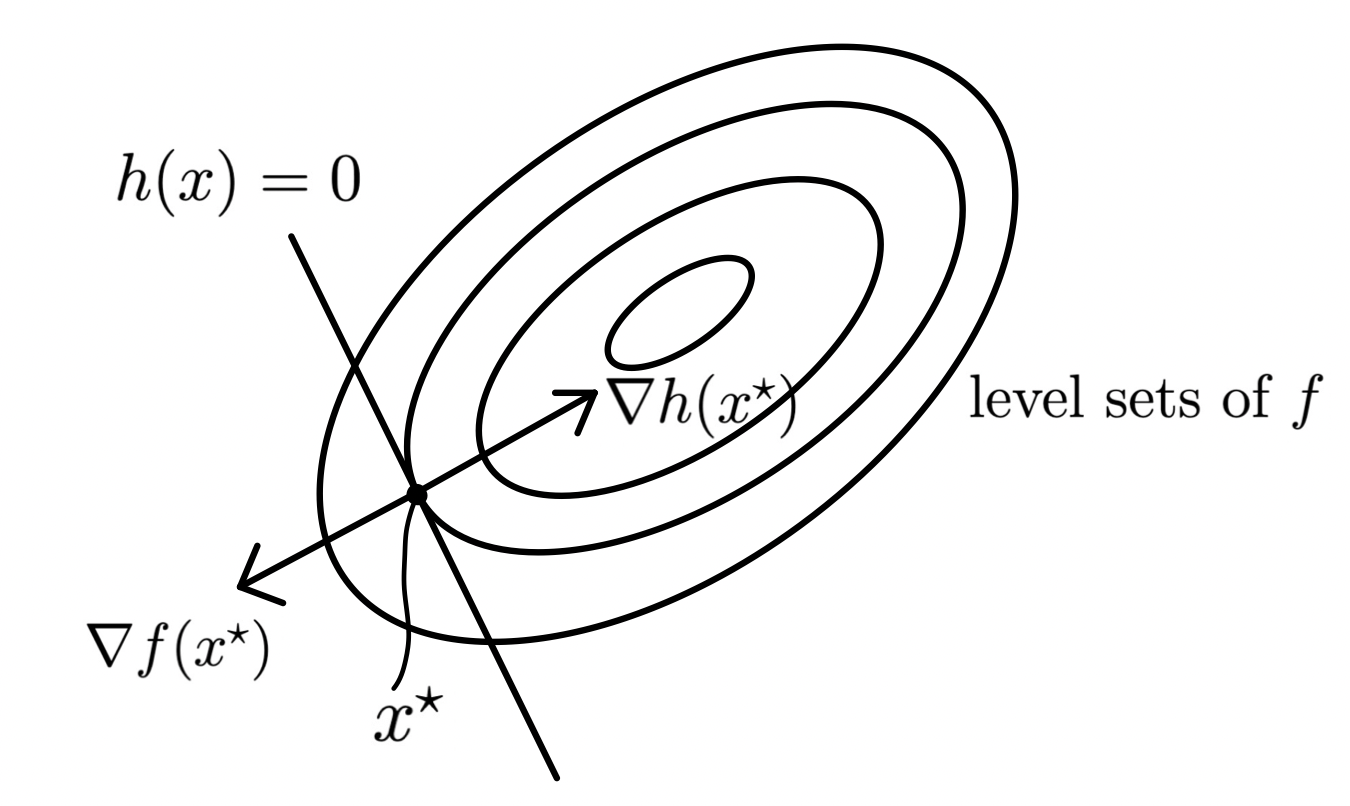
\includegraphics[width=\columnwidth]{images/op_eq_constraints.png}

We note the following:
$\nabla f(x^\star)$ and $\nabla h(x^\star)$ are colinear

$\Leftrightarrow$
$\exists\ \nu^\star \in \mathbb{R}: \nabla f(x^\star)+\nu^\star\nabla
h(x^\star) = 0$

$\Leftrightarrow$
$f(x)+\nu^\star h(x)$ is stationary at $x^\star$,
where $\nu^\star$ can be interpreted as cost of violationg constraint

\subsection{Generalization}

Consider
\[
  f^*=\inf_x f(x)\quad\text{s.t.}\quad h(x)=0,\;g(x)\le 0.
\]
The Lagrangian is
\[
  \mathcal{L}(x,\lambda,\nu)=f(x)+\lambda^\top g(x)+\nu^\top
  h(x),\qquad\lambda\ge 0.
\]

\subsection{Weak Duality}
\(d(\lambda,\nu)=\inf_x\mathcal{L}(x,\lambda,\nu)\le f^*\) for all
feasible multipliers.

\subsection{Strong Duality}
If the problem is convex and Slater’s condition holds
(\(\exists\hat{x}\) with \(g(\hat{x})<0\), \(h(\hat{x})=0\)), then
there exist \(\lambda^*\ge 0\), \(\nu^*\) such that \(d(\lambda^*,\nu^*)=f^*\).

\subsection{KKT Optimality Conditions}
Under convexity + Slater, \(x^*\) is primal optimal and
\((\lambda^*,\nu^*)\) is dual optimal if and only if
\begin{align*}
  \nabla_x\mathcal{L}(x^*,\lambda^*,\nu^*)&=0 &&\text{(stationarity)},\\
  g(x^*)&\le 0,\;h(x^*)=0 &&\text{(primal feasibility)},\\
  \lambda^*&\ge 0 &&\text{(dual feasibility)},\\
  \lambda^{*\top}g(x^*)&=0 &&\text{(complementary slackness)}.
\end{align*}
The last equality together with strong duality yields
\[
  \sup_{\lambda\ge 0,\nu}d(\lambda,\nu)=\inf_{x\in\mathcal{C}}f(x).
\]

\subsection{Subdifferential (Nonsmooth Case)}
For a convex function the subdifferential at \(\bar{x}\) is
\[
  \partial f(\bar{x})=\{\,v\mid f(x)\ge
  f(\bar{x})+v^\top(x-\bar{x})\;\forall x\,\}.
\]
A point \(x^*\) minimises \(f\) if and only if \(0\in\partial
f(x^*)\). When \(f\) is differentiable we recover the classical
gradient condition.

